\begin{frame}{Probabilistic Modeling}

%source:https://texample.net/tikz/examples/connecting-text-and-graphics/


\begin{columns}
    \begin{column}{0.48\textwidth}
        \centering
        \begin{bmatrix}
        0 &  &  &  &  &  &  &  &  &  \\ 
        0 & 0 &  &  &  &  &  &  &  &  \\ 
        \vdots & \vdots & \vdots & \vdots & \vdots & \vdots & \vdots & \vdots & \vdots & \vdots \\
        1 & 1 & 1 & 1 & 1 & 0 \tikz[na] \coordinate (s-69); & 1 & 1 & 0 &   \\ 
        1 & 1 & 0 \tikz[na] \coordinate (s-310); & 1 & 1 & 1 & 1 & 1 & 1 & 0 \\ 
        \end{bmatrix}
    \end{column}
    \begin{column}{0.48\textwidth}
        \tikzstyle{background grid}=[draw, black!50,step=.5cm]
        \begin{tikzpicture}%[show background grid]
            % Put the graphic inside a node. This makes it easy to place the
            % graphic and to draw on top of it. 
            % The above right option is used to place the lower left corner
            % of the image at the (0,0) coordinate. 
            \node [inner sep=0pt,above right] 
                {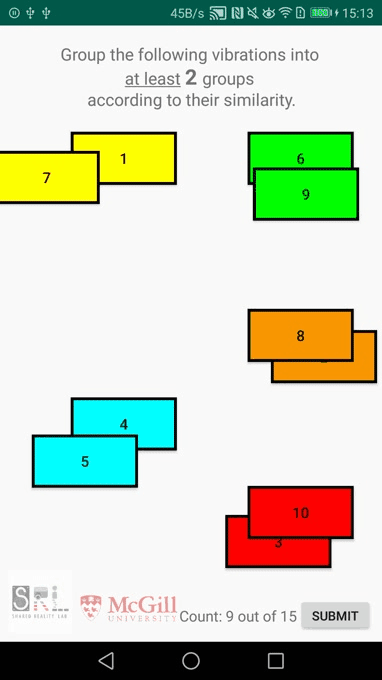
\includegraphics[width=4cm]{Images/3.png}};
            % show origin
            % \fill (0,0) circle (2pt);
            % define destination coordinates
            \path (2.5,5.3) coordinate (im69)
                  (2.3,1.3) coordinate (im310);
        \end{tikzpicture}
    \end{column}
\end{columns}

% define overlays
% Note the use of the overlay option. This is required when 
% you want to access nodes in different pictures.
\begin{tikzpicture}[overlay]
        \path[<-,green,thick] (s-69) edge [bend left] (im69);
        \path[<-,red,thick] (s-310) edge [bend right] (im310);
\end{tikzpicture}


\end{frame}